% !TEX TS-program = pdflatex
% !TEX encoding = UTF-8 Unicode

% "dictionary": "Packages/User/Swedish.dic",

\documentclass[a4paper]{article}

\usepackage[swedish]{babel}
\usepackage[T1]{fontenc}
\usepackage[utf8]{inputenc}
\usepackage[pdftex]{graphicx}
\usepackage{float}
\usepackage{fancyhdr}
\usepackage[toc,page]{appendix}
\usepackage{listings}
\usepackage{booktabs} % for much better looking tables
\usepackage{array} % for better arrays (eg matrices) in maths
\usepackage{paralist} % very flexible & customizable lists (eg. enumerate/itemize, etc.)
\usepackage{verbatim} % adds environment for commenting out blocks of text & for better verbatim
\usepackage{subfig} % make it possible to include more than one captioned figure/table in a single float
\usepackage[margin=2.5cm]{geometry}

\usepackage[stable]{footmisc} % footnotes in section tags
\usepackage{natbib} % automatic short-hand citations

%%% Custom chapter and section style
\usepackage{titlesec, blindtext, color}
\definecolor{gray75}{gray}{0.75}
\newcommand{\hsp}{\hspace{20pt}}

\usepackage{sectsty}
\allsectionsfont{\sffamily\mdseries\upshape} % sans serif headings

\setlength{\parindent}{0pt}

%%% HEADERS & FOOTERS
\author{Niclas Olofsson}
\pagestyle{fancy} % options: empty , plain , fancy
\renewcommand{\headrulewidth}{1pt} % customise the layout...
\fancyhead[LO,L]{Niclas Olofsson\\Designdokument}
\lfoot{}\cfoot{\thepage}\rfoot{}

\title{Designdokument\\Bemanning i GOLI Kapacitetsplanering}

\begin{document}
\maketitle

\section{Inledning}
GOLI Effektivitetsplanering är ett system för produktionsplanering,
vilket används för att planera och följa upp produktionen i en viss
verksamhet. Ett exempel kan vara en röntgenavdelning på ett sjukhus, där
man planerar att göra ett visst antal undersökningar per dag. Vissa
dagar lägger man in extrapass med syftet att korta ner vårdköerna, och
vissa dagar måste röntgenmaskinen genomgå underhåll. Detta leder till
planerade variationer i antalet undersökningar över tid, vilka kan
följas upp genom att jämföra det planerade antalet med hur många
undersökningar som faktiskt gjordes. På grund av efterfrågan från kunder
vill GOLI utöka sin tjänst till att även innefatta stöd för hantering av
bemanning.\\

Syftet med detta dokument är att beskriva funktionaliteten i den tänkta
utökningen av systemet enligt de önskemål som kommit från kunder, samt
beskriva en plan för utveckling, tester och implementation av denna.\\


\section{Bakgrund}
During code refactoring or implementation of new features in software,
errors often occur in existing parts. This may have a serious impact on
the reliability of the system, thus jeopardizing user's confidence for
the system. Automatic testing is utilized to verify the functionality of
software in order to detect bugs and errors before they end up in a
production environment.\\

Starting new web application companies often means rapid product
development in order to create the product itself, while maintenance
levels are low and the quality of the application is still easy to
assure by manual testing. As the application and the number of users
grows, maintenance and bug fixing becomes an increasing part of the
development. The size of the application might make it implausible to
test in a satisfying way by manual testing.\\

The commissioner body of this project, GOLI, is a startup company
developing a web application for production planning called GOLI
Kapacitetsplanering. Due to requirements from customers, the company
wishes to extend the application to include new features for handling
staff manning. The current system uses automatic testing to some extent,
but these tests are cumbersome to write and takes long time to run. The
purpose of the thesis is to analyze how this application can begin using
tests in a good way whilst the application is still quite small. The
goal is to determine a solid way of implementing new features and bug
fixes in order for the product to be able to grow effortlessly.\\


\section{Metodik}
Då examensarbetets fokus är testning och testbarhet, kommer testdriven
utveckling (TDD) att användas vid implementationen av den nya
funktionaliteten, med vissa inslag från behaviour-driven development
(BDD). Syftet med detta är att få en bild av hur väl detta fungerar i
praktiken, samt vilka svårigheter och utmaningar som finns vid testning
av webbaserade applikationer. Automatiska systemtester kommer att göras
med Selenium och Capybara, unit-tester med RSpec och Jasmine. Själva
implementationen kommer att ske i Ruby och CoffeScript med ramverken
Ruby on Rails 4 och KnockoutJS 3, med MongoDB som DBMS, då detta är de
teknologier som används i det befintliga systemet.\\


\section{Systemdesign}

\subsection{Datamodeller}

\begin{figure*}[t]
\centering
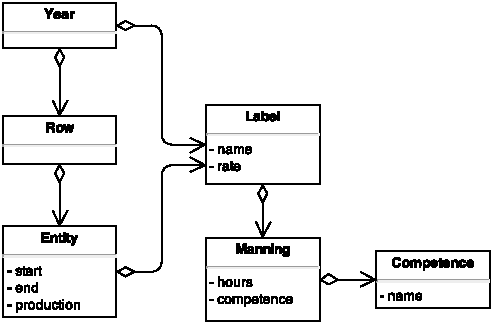
\includegraphics[width=0.6\textwidth]{model.pdf}
\caption{UML-diagram för de relevanta delarna av systemet}
\label{fig:model}
\end{figure*}

Ett förenklat UML-diagram för de relevanta delarna av systemet visas i
Figur \ref{fig:model}. Tanken är att den befintliga datamodellen i
framtiden kan utökas med klassen \emph{Manning}. Ett sådant objekt
representerar en bemanning som krävs för en viss typ av aktivitet, t.ex.
en viss typ av personal som ska jobba ett visst antal timmar. I
framtiden kan varje sådan bemanning även kräva en eller flera
kompetenser.\\

Uppdragsgivaren vill undvika en onödigt komplicerad datastruktur i den
händelse att systemet inte kommer att utökas med mer komplexa krav på
modellen. Därför kommer till en början ett attribut på klassen
\emph{Label} att användas för att beskriva antalet bemannade timmar,
istället för att utöka datamodellerna med en ny klass. Skapandet av en
separat \emph{Manning}-klass skulle i så fall kräva en mindre
datamigrering.\\

Om det finns ett behov av att följa upp faktisk bemanning, kan detta
lösas med ett nytt attribut för antal bemannade timmar på klassen
\emph{Entity}.


\subsection{Användargränssnitt}

Vi tror att det smidigaste alternativet är att kunna byta mellan olika
lägen i användargränssnitten, beroende på om man vill visa planerad
bemanning eller planerad produktion. En svårighet är att representera
detta på ett bra sätt för användaren, då till synes likadana siffror
då får radikalt olika betydelse beroende på i vilket läge man befinner
sig. Därav kommer framtagningen av gränssnittet ske iterativt, där
olika versioner kan utvärderas i samarbete med systemets användare.\\

En central del är den totala summan av antalet bemannade timmar. Detta
tillhandahålls i användargränssnittet som en möjlighet att se
summeringar för timmarna. Det vore troligen lämpligt att kunna summera
dessa såväl totalt och per veckodag som per aktivitet.\\



%\section{Nuvarande design}
%\input{current.tex}

\end{document}
